\documentclass[../main.tex]{subfiles}
\graphicspath{{\subfix{../IMAGES/}}}

\begin{document}
\localtableofcontents
\subsection{Preprocessing of images}
An image is a function of 2 spatial variables. 2D images : m=2, monochromatic images, digital images : discrete domain. \\
For monocromatic images : 1scalar/pixel. Often displayed as grey levels, choice of other color lookup tables. \\
Multi-spectral images : 1vector/pixel (ex : color images, each pixel has three color component).\\

Fourier transform of a 2D signal : it is separable ($F_x = \int_{-\infty}^\infty f(x,y) e^{-j2\pi f_x x}dx$).\\
Sampling a continuous function means taking samples at every $\Delta x$ and $\Delta y$. Mathematically, it is the multiplication of an analog image by a grid of Dirac impulses. The spectrum of the sampled image can be obtained by a convolution of the spectrum of the analog image with the FT of the grid of Dirac impulses. One can try to reconstruct the original image by low pass filtering (multiply the spectrum by a rectangle function and convolve the sampled image by a signal of type $\frac{sin(x)}{x}$).\\
If aliasing : low-pass filtering and interpolation. \\
It is possible to perform geometrical operations on images as a preprocessing step : \begin{itemize}
    \item translation : thanks to interpolation, it is possible to reconstruct an image translated by a non-integer number of pixels (inverse translation + interpolation) : $\begin{pmatrix}
        x\\y\\
    \end{pmatrix} = \begin{pmatrix}
        u\\v\\
    \end{pmatrix} + \begin{pmatrix}
        t_x\\t_y\\
    \end{pmatrix}$
    \item rotation : same 
    \item Linear/non linear transformations : always start with the inverse transformation. 
\end{itemize}

\subsubsection{Histogram equalization}
The goal is to create an image with a uniform histogram by transformation $q=T(p)$.\\
Input histogram : $G(q_i) = \frac{N^2}{q_i-q_0}$, output : $H(p_i)$.\\
$\sum G(q_i) = \sum H(p_i)$. Then : $q = T(p) = \frac{q_k-q_0}{N^2} \sum^p_{p_0} H(i) + p_0$.\\
\warning As the colors are changed it only serves a purpose to see better the image it does not help with quantification.\\

\subsubsection{Denoising}
Source of noise in images : interferences on the measurements, signal quantification. Characteristics of the noise : random signal, additive and Gaussian : $y(t) = x(t)+n(t)$.\\
The \textbf{importance of the noise} is the signal to noise ratio : $SNR = 10\log \frac{P_s}{P_N}$.\\
In general, the noise has zero mean : take multiple pictures and average the results to remove the noise.\\
If only access to one image : filters!\\
A low-pass filter reduces the noise but can alter the image too : $G(i,j) = \sum_m \sum_n F(m,n) H(m-i, n-j)$.\\
Some simple ones : $H = \frac{1}{9} \begin{pmatrix}
    1 & 1 &1\\ 1 & 1 &1 \\ 1&1&1\\
\end{pmatrix}$, $H = \frac{1}{10} \begin{pmatrix}
    1 & 1 &1\\ 1 & 2 &1 \\ 1&1&1\\
\end{pmatrix}$\\
\warning It also blurs the image.\\

One can use a \textbf{homomorphic filter} : noise is multiplicative and depends on intensity of the signal. Model of the image : $f_0(i,j) = f_i(i,j) n(i,j)$. One can make it additive by taking the log.\\

One can also use non-linear filtering : \\
\textbf{outliers} : compare the pixel value with mean of the neighbors and remove it if above a certain threshold. (conditional convolution with $H = \frac{1}{8} \begin{pmatrix}
    1 & 1 &1\\ 1 & 0 &1 \\ 1&1&1\\
\end{pmatrix}$).\\
\textbf{median filter} : let's consider the neighbors of a picel on a neighborhood of size nxn. Let's sort the values of those pixels in ascending order and set the median value of this list as the value of the current pixel.\\
\warning It suppresses the small variations and keeps the contours.\\

\quad \underline{Contour enhancement :}\\
Enhance the high frequencies : filtering by a high pass filter ($H = \begin{pmatrix}
    0 & -1 &0\\ -1 & 5 &-1 \\ 0&-1&0\\
\end{pmatrix}$).\\

\quad \underline{Image restoration :}\\
Invert non-wanted effects. Typical application : deconvolution.\\
The goal is to restore the initial image using a model for the original image and for the noise. Let the ideal image $f_i$ be degrated bby an undesired filtering effect and $f_o$ the observed image : $f_o = f_i ** h_D + n$.\\
One needs to find the inverse filter : $h_r$ such that $\hat{f}_i = f_o ** h_r$.\\
A naive solution is to take an inverse filter : $H_R = \frac{1}{H_D}$ (in the Fourier domain), but the restored image is : $\hat{F}_i = F_i + \frac{N}{H_D}$. If the image is clean, it works well! Otherwise, it will increase the noise and make the signal unstable.\\
Another solution : \textbf{Wiener filter}.\\
Goal is to find a filter $h_r$ that minimizes the quadratic error ($\varepsilon = E\{[f_i-\hat{f}_i]^2  \}$). By FT, we obtain $H_r = \frac{P_{f_i,f_o}}{P_{f_o}}$, $P_{f_i,f_o}$ the power interspectrum, $P_{f_o}$ the power spectrum of $f_o$. This can be rewritten as : \begin{equation}
    H_r(\omega_x, \omega_y) = \frac{H_D^*(\omega_x, \omega_y)}{\lvert H_D^*(\omega_x, \omega_y)\rvert^2 + \frac{P_N(\omega_x, \omega_y)}{P_{f_i}(\omega_x, \omega_y)}}
\end{equation}
Wiener filter is an adaptive band-pass filter. Behaves as an inverse filter at low frequencies and low-pass filter at high frequencies.
$h_D$ is the impulse response of the system. Thus if we find in the image a punctual object, one can deduce $h_D$. A uniform region in the image shows the noise. The FT of its autocorrelation gives an estimation of the power spectrum of the noise. 

\subsection{Image segmentation}
In practice, objects are often connex, with coherent color and/or surrounded by sharp contours.\\
Segmentation is the partition of an image in a finite number of regions such that : $R\cup R_i$, $R_i \cap R_j = \emptyset$, $i\neq j$.\\
Two methods : region-based segmentation and contour-based.\\

\subsubsection{Region-based segmentation}
Separation of the image into regions by setting threshold on gray levels. i.e : $g(i,j) = \begin{cases}
    1 & f(i,j)\geq T\\ 0 & f(i,j)<T
\end{cases}$. How to find the optimal threshold(s)?\\

\begin{itemize}
    \item Based on the image histogram : choice of the threshold that minimizes the segmentation error. Identify the two main maxima and take the minimum in between. \warning Avoid to consider two local maxima that belong to the same mode.
    \item Based on the histogram with optimal thresholding : gray level distributions can often be modeled with Gaussian. The optimal threshold is the point of intersection of the gaussian distributions. The threshold is such that : $\mathcal{P}(\omega_1,x_T) = \mathcal{P}(\omega_2,x_T)\Rightarrow \mathcal{P}(x\lvert \omega_1) \mathcal{P}(\omega_1) = \mathcal{P}(x\lvert \omega_2) \mathcal{P}(\omega_2)$. Model the histogram with two gaussians : $d(l) = A e^{-\frac{(l-c)^2}{2\sigma^2}}$ and fit them. The function to optimize is then : $\varepsilon = \frac{1}{1+l_{max}} \sum_l^{l_{max}} [h(l) - (d_b(l)+d_o(l))]^2$.  
\end{itemize}

Segmentation by thresholding is very simple and work well but in a limited number of cases. It does not define objects but separates background from foreground $\Rightarrow$ region growing methods.\\

\quad \underline{Region growing :}\\
Let's fix a starting point (seed) in the desired region. Let's define the \textbf{homogeneity criterion} used to define the region. By a recursive procedure, it includes in the region all the pixels that are neighbors of the current pixel and that satisfy the homogeneity criterion. We obtain a connex region. The homogeneity criterion can be : intensity varies slowly, local variance is lower than a threshold...

\quad \underline{Region merging :}\\

It consider each pixel as a region and fuses adjacent regions if the homogeneity criterion of the union is respected. \warning Result depends on the order of the fusion process. Often : rough segmentation. \\
Joins multiply regions.

\quad \underline{Region splitting :}\\
Opposite, divide regions. It divides the image when the homogeneity criterion is not met.\\
\warning Often : over-segmentation.\\

\quad \underline{Split and merge :}\\
One starts by splitting the image into small homogeneous regions and regroups them.\\


\subsubsection{Contour-based segmentation : edge detection}
The other way to define a region is to search for sharp edges : contour based methods. An edge is : a sharp transition of intensity in an image (intensity profile is a step function, first derivative has a maximum, second derivative crosses zero).\\

\begin{figure}[hbt!]
    \centering
    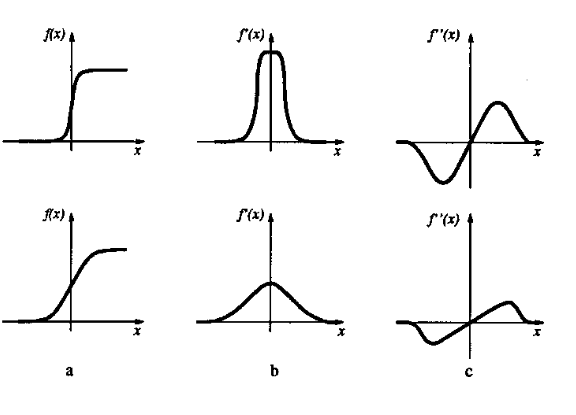
\includegraphics[width=0.5\linewidth]{IMAGES/Indus_el/Screenshot from 2025-03-02 19-33-34.png}
\end{figure}

\quad \underline{Maximum of the 1st derivative :}\\
Filter that approximate first derivative : 
\begin{itemize}
    \item Robert operator : $h_1 = \begin{pmatrix}
        1 & 0\\ 0 &-1
    \end{pmatrix}$ and $h_2 = \begin{pmatrix}
        0 & 1\\ -1 & 0
    \end{pmatrix}$
    \item Prewitt : $h_1 = \begin{pmatrix}
        1 & 1 & 1\\0&0&0\\-1&-1&-1
    \end{pmatrix}$, $h_2 = \begin{pmatrix}
        0&1&1\\-1&0&1\\-1&-1&0
    \end{pmatrix}$ and $h_3 = \begin{pmatrix}
        -1&0&1\\-1&0&1\\-1&0&1
    \end{pmatrix}$
\end{itemize}

\quad \underline{Zero-crossing of the 2nd derivative :}\\
Laplacian of Gaussian. Noise introduces false detections. Let's filter the image to remove the noise and undesired details : Gaussian filter.\\
Trick is to exploit the property of convolution : $\nabla^2 (G(x,y)**f(x,y))= (\nabla^2 G(x,y))**f(x,y)$, $G(x,y) = e^{-\frac{x^2+y^2}{2\sigma^2}}$ (the bigger the sigma, the bigger the smoothing) $\Rightarrow$ one has to convolve the image by the second derivative of a Gaussian and find the zero crossing of the resulting image.\\ 

\warning If an image is too noisy : fill the holes and smooth the borders after segmentation.\\

\subsubsection{Mathematical morphology}
The principle is to compare the objects present in an image with a reference object, of given size and shape, called structuring element. \\
A translation is defined as : $(A)_x = \{c\in E \lvert c=a+x, \forall a\in A\}$. A dilation is : $X\oplus B = \{c\in E \lvert c=a+b, a\in X, b\in B\} = \cup_{b\in B} (X)_b$. An erosion is : $X\ominus B = \{c\in E \lvert \forall b\in B, c+b\in X\} = \cap_{b\in B} (X)_{-b}$ (dual of the dilation : if you dilate$X\ominus B$ you get something included in X).\\
One does not want to dilate the object, therefore one has to erode it first and dilate it then : opening $X\circ B = (X\ominus B)\oplus B$, the opposite is closing : $X\cdot B = (X\oplus B) \ominus B$.\\

Few rules : extensivity (if $0\in B$, $A\subseteq A\oplus B$), increasing ($A\subseteq B \Rightarrow A\oplus C \subseteq B\oplus C$), $(A\cup B)\oplus C = (A\oplus C) \cup (B\oplus C)$, $(A\cap B) \oplus C \subseteq (A\oplus C)\cap (B\oplus C)$, anti-extensivity (if $0\in B$, $A\ominus B\subseteq A$), invariance by translation ($(A)_x \ominus B = (A\ominus B)_x$, $A\ominus (B)_x = (A\ominus B)_{-x}$), increasing ($A\subseteq B \Rightarrow A\ominus K \subseteq B\ominus K$), $A\ominus (B\oplus C) = (A\ominus B)\ominus C$.\\

Reflection of B : $\overline{B} = \{x \lvert -x\in B\}$. \textbf{Duality erosion dilation :} $(A\ominus B)^c = A^c \oplus \overline{B}$. Which can be translated to : the background of an erosion is the dilation of the background. \\

Then properties : duality ($X\circ B = (X^c \cdot \overline{B})^c$), extensivity ($X\circ B\subseteq X$ and $X\subseteq X\cdot B$), idempotence ($(X\circ B)\circ B = X\circ B$, $(X\cdot B)\cdot B = X\cdot B$).\\
Erosion an dilation change the size of the objects. Opening and closing : fill the holes (inside the objects : closing, external to the objects : opening).



\end{document}